%%%%%%%%%%%%%%%%%%%%%%%%%%%%%%%%%%%%%%%%%%%%%%%%%%
%%%%		~~~~ Appendix example ~~~~
%%%%%%%%%%%%%%%%%%%%%%%%%%%%%%%%%%%%%%%%%%%%%%%%%%

\chapter{Appendix}
% START APPENDIX
\section{Comparing Tokenization lengths}
\label{tok_compare}
Pretokenized Sequence Lengths - Mean: 47976.146146146144, Median: 43692.0, Std Dev: 23159.918513030065
Tokenized Sequence Lengths - Mean: 14519.587587587588, Median: 13159.0, Std Dev: 7197.064427699848

Applying the BPE tokenizer results in sequence lengths roughly 1/3 of the original sequences. The sample is taken from 1000 random music pieces from the lakh-midi dataset. 

\begin{figure}[H]
    \centering
    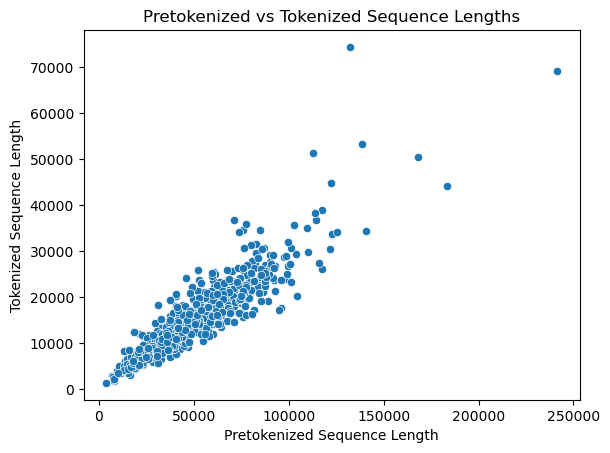
\includegraphics[width=0.5\textwidth]{IMAGES/scatter_pre_post_tok.png} 
    \caption{Scatterplot of Pre-tokenization vs bpe-tokenization sequence lengths}
    \label{fig:tok_compare}
\end{figure}


\section{Integration into LastMinuteGig 2 months}
This project is motivated by extending the music engine of LastMinuteGig. \cite{Chalkiadakis_2022}. The application currently employs a very simple algorithm. I will outline it below. 
\begin{itemize}
    \item{1}: Randomly choose key, rhythmic pattern, chord progression and tempo from a pool of possible values.
    \item{2}: Play corresponding percussion audio clip (depends on tempo and rhythmic pattern)
    \item{3}: When user plays the button trigger the guitar sound of the current chord.
    \item{4}: After 8 bars - make a random change (to rhythm, tempo, pause)
\end{itemize}


This music engine will be changed in the following way. Most of the generative process will be done asynchronously.
\begin{itemize}
    \item{1}: Create $n=100$ musical pieces with different control settings
    \item{2}: For each piece
    \item{3}: Extract chords from prompt (assuming high control success) - save mapping $m1$
    \item{4}: Extract change of rhythmic pattern (or tempo or meter or instrumentation since these are already controllable in the musiclang model) - save mapping
    \item{5}: Render symbolic music to audio
\end{itemize}

During game play
\begin{itemize}
    \item{1}: Load random audio clip and mappings.
    \item{2}: Play associated guitar chords when player taps.
    \item{3}: Register changes in tapping on musical changes.
    \item{4}: Repeat when audio clip has finished playing.
\end{itemize}

\begin{table}[H]
\label{table:bigtable}
    \centering
    \begin{tabular}{|l|l|l|l|l|l|l|}
        \hline
        \textbf{Name} & \textbf{Architecture} & \textbf{Control} & \textbf{FG} & \textbf{MI} & \textbf{Dataset} & \textbf{Representation} \\
        \hline
        DeepBach (2017) \cite{Hadjeres_Pachet_Nielsen_2017} & RNN & Inpainting & Yes & Yes & \cite{jsbchorales} & Midi-Like\\ 
        FolkRNN (2015) \cite{Sturm_Ben-Tal_2016} & RNN & meter, mode & No & No & \cite{sessionfolkdata} & REMI-Like\\
        MT (2018) \cite{Huang_Vaswani_Uszkoreit_Shazeer_Simon_Hawthorne_Dai_Hoffman_Dinculescu_Eck_2018} & Transformer & - & No & No & \cite{hawthorne2018maestro} \cite{jsbchorales} & Midi-Like\\
        MidiNet (2019) \cite{midinet} & GAN & chords, melody & Yes & Yes & \cite{hooktheorypopmidi} & Midi-Like\\
        Polyfussion 2023 \cite{Min_Jiang_Xia_Zhao_polyffusion_2023} & Diffusion &inpainting),texture & Yes & No & \cite{Wang_Chen_pop90_dataset} & Piano-Roll\\
        FIGARO 2023 \cite{Rütte_figaro_2023} & Transformer & chords, instr, meter, nd & Yes & Yes & \cite{Raffel_2016} & REMI+ \\
        MMT 2023 \cite{Dong_Chen_MMT_Kirkpatrick_2023} & Transformer & instrumentation & No & Yes & \cite{Raffel_2016},\cite{Crestel_OrchestralDataset} & Midi-Tuple \\
        OMT 2020 \cite{Huang_Yang_remi_pop_transformer_2020} & Transformer & chords, tempo & Yes & No & C & REMI\\
        MuseNet 2019 \cite{Christine_2019} & Transformer & instr, genre & Yes & Yes & \cite{hawthorne2018maestro}\cite{classicalarchives}\cite{bitmidi} & ?\\
        MMM 2020 \cite{Ens_Pasquier_2020_MMM} & Transformer & inpainting, instr, nd & Yes & Yes & \cite{Raffel_2016} & C\\
        Sympack 2024 \cite{Chen_Smith_Spijkervet_Wang_Zou_Li_Kong_Du_2024} & Transformer & chords, structure, notes& Yes & Yes & \cite{Raffel_2016} \cite{Bertin-Mahieux_Ellis_Whitman_Lamere_2011}, C &  \\
        MuseCoco 2023 \cite{Lu_Xu_Kang_Yu_Xing_Tan_Bian_MuseCoco_2023} & Transformer & various & No & No & C & REMI-Like\\
        MBC 2024 \cite{Shu_Xu_Musebarcontrol_2024} & Transformer & chords & Yes & No & \cite{Wang_Chen_pop90_dataset} & REMI-Like\\
        Museformer 2022 \cite{Yu_Lu_Wang_Hu_Tan_Ye_Zhang_museformer_2022} & Transformer & - & No & Yes & \cite{Raffel_2016} & REMI-Like\\
        NTT \cite{Ryu_Dong_nested_2024} & Transformer & - & No  & Yes & \cite{Raffel_2016} \cite{Wang_Chen_pop90_dataset} \cite{Crestel_OrchestralDataset} & Compound\\
        FTG \cite{Zhu_Liu_Jiang_Zheng_texture_2024} & Diffusion & texture, rhythm, chords & Yes & No & \cite{Wang_Chen_pop90_dataset} & Piano-Roll \\
        Fader Nets & VAE & rhythm, arousal & No & No & \cite{hawthorne2018maestro} & Perf \\
        NDRD \cite{Huang_rule_diffusion_2024} & Diffusion & chord, pitch, nd & Yes & No & \cite{hawthorne2018maestro} \cite{Wang_Chen_pop90_dataset} & Piano-Roll \\
        \hline
    \end{tabular}
    \caption{Overview of music generation models, their architectures, and control mechanisms. Empty columns indicate missing information on fine-grained control, multitrack capabilities, dataset, and evaluation methods.}
    \label{tab:music_models}
\end{table}

\section{Notes Comparing Symbolic Music Generators and their evaluation methods}
\label{section:compare_sym}
\begin{itemize}

\item DeepBach \cite{Hadjeres_Pachet_Nielsen_2017} - RNN - inpainting. Evaluation Turing
\item FolkRNN \cite{Sturm_Ben-Tal_2016} - RNN - control for meter and mode - Expert Evaluation + Performance Practice
\item MusicTransformer \cite{Huang_Vaswani_Uszkoreit_Shazeer_Simon_Hawthorne_Dai_Hoffman_Dinculescu_Eck_2018} - Transformer - Evaluation: Subjective - Tournament Style between different generated and natural music. Objective: Validation NLL
\item MidiNet\cite{midinet} - GAN - Control for Chords/Priming melody.
 Human (how pleasing, how real, and how interesting)

\item Polyfussion \cite{Min_Jiang_Xia_Zhao_polyffusion_2023} - Diffusion Model - supports inpainting, interpolation, melody/accompaniment generation, control for chord progression, texture. Subjective Evaluation Questionnaire for naturalness, creativity, musicality. Objective Control success. 

\item FIGARO \cite{Rütte_figaro_2023} - Transformer Model - bar-wise control for chords, instrumentation, time-signature, note-density, mean-pitch. 
Evaluation: Perplexity (improvement over NLL for sequences of different length), Discription Fidelity (i.e accuracy in regards binary controls instruments, chords, time-signature). Macro Overlapping Area - comparison of feature histograms. Normalized Mean Root Square Area for note-density. Cosine similarity for chroma (melodic) and groove (rhythmic) feature vectors. 
Ablation study - effect of turning off controls.
Extensive Subjective evaluation:  7569 comparisons by 691 participants - tournament style.

\item Multi Track Music Transformer  (MMT) \cite{Dong_Chen_MMT_Kirkpatrick_2023}  - Transformer - Instrument control. Comparison of different tokenisation techniques, REMI+ and Compound Tokens. Compound tokens are more condensed and the generated samples are longer, achieves significant speedups and reduces memory usage (2.6 * MMM, or 3.5 * REMI+). Objective evaluations: Inference time, pitch class entropy, scale consistency, groove consistency, 
Human evaluation (90 comparisons by 9 participants) on Coherence Richness Arrangement Overall.

Additional: Analysis of self attention as explanation avenue, which notes are most important. 

\item REMI pop music transformer - \cite{Huang_Yang_remi_pop_transformer_2020} - Transformer - continuation, control local control over chord and tempo

\item MuseNet \cite{Christine_2019} - Transformer -,Instrument control, style control. No evaluation, only showcase.

\item MMM \cite{Ens_Pasquier_2020_MMM} - Transformer model - inpainting, instrument control, note-density.
Introduce novel representation
No Rigorous Evaluation 

\item SymPAC \cite{Chen_Smith_Spijkervet_Wang_Zou_Li_Kong_Du_2024}  - Transformer - Control for Chords, structure, instrumentation, single notes.
Train with both symbolic and transcribed audio data.
Fine grained control. Constrained generation with a Finite State Machine. 
Comparison of three separate models trained on three datasets.
\textbf{Evaluation} of controlability with KL-divergence on different controlled features over chords, structure, and individual notes. - KL divergence decreases with dataset size. 800 samples are generated and compared against a validation set of 3000 songs. 
Subjective evaluation (12 expert participants MIR researchers and music producers) on parameters of Coherence Richness Arrangement Structure 

\item MuseCoco \cite{Lu_Xu_Kang_Yu_Xing_Tan_Bian_MuseCoco_2023} - Transformer - Control via text for following attributes instrumentation, ambitus, rhythm (intensity and “dancability”), number of bars, time signature, key, tempo, duration, artist, emotion, genre. All of these controls are global controls, a description is converted into a list of  attributes which is then used for generation. 
Combination of many datasets. Creation of text descriptions from attribute list with data from the dataset, and ChatGPT. 
Evaluation: Objective - text to attribute list. 
Subjective evaluation 19 participants with at least basic music knowledge - questions to Musicality, Controlability (adherence of sample to music description), Overal Impression. Comparison with LLM generated music (with no special training for music generation)

\item MBD \cite{Shu_Xu_Musebarcontrol_2024} Extension of MuseCoco for time varying chord controls. Counterfactual Loss and Auxiliary task training improve controllability. 

\item{Museformer} \cite{Yu_Lu_Wang_Hu_Tan_Ye_Zhang_museformer_2022} - Transformer - No controls. Goal improve long-term structure with fine and coarse attention. Captures structure well. 
Objective Evaluation: Perplexity: prediction accuracy of next token, Similarity Error the error between the similarity distribution of training data and generated
music 
Subjective Evaluation 10 Participants Musicality, Long Term Structure, Short Term Structure.
Ablation study - evaluate objective effect of coarse and fine-grained attention. + Case study and detailed look at model.

\item{NMT} \cite{Ryu_Dong_nested_2024} - Transformer improve longterm structure and reduce sequence length through compound tokens. Application to both symbolic and audio tokens. 
Cross attention vs self-attention comparison 
Evaluation: FAD, CLAP, KL and NLL over audio tokens. NLL over symbolic tokens. 
Subjective Evaluation Coherence, Richness, Consistency, Overall 29 participants. 8 selected prompts, 4 different continuations with REMI, Compound Word and 2 NMT variations.


\item{FTG - Fine Grained Texture Control} - Diffusion - control over texture, rhythm and chords. 

\item{Fader Nets}\cite{Tan_Herremans_2020} - VAE - Control over rhythm, arousal, 
Idea: develop a "fader" representing a high-level abstract feature i.e arousal. Arousal is disentangled using a VAE into lower level features (i.e rhythmic density).

Evaluation of the influence of latent features is on generated (style transfer) music.:
Consistency, Restrictiveness (one latent dimension does not influence other musical features), Linearity (linear change in latent feature - linear change in musical feature)
Subjective listening test to indicate success of arousal shift -> 48 participants, evaluate agreement with arousal direction. 

\item{NDRD} Symbolic Music Generation with Non-Differentiable Rule Guided Diffusion.
Guidance of diffusion sampling with non-differentiable rules. 
\end{itemize}
